%% ----------------------------------------------------------------
%% Thesis.tex -- MAIN FILE (the one that you compile with LaTeX)
%% ---------------------------------------------------------------- 

% Set up the document
\documentclass[a4paper, 11pt, oneside]{Thesis}  % Use the "Thesis" style, based on the ECS Thesis style by Steve Gunn
\graphicspath{Figures/}  % Location of the graphics files (set up for graphics to be in PDF format)

% Include any extra LaTeX packages required
\usepackage[square, numbers, comma, sort&compress]{natbib}  % Use the "Natbib" style for the references in the Bibliography
\usepackage{verbatim}  % Needed for the "comment" environment to make LaTeX comments
\usepackage{vector}  % Allows "\bvec{}" and "\buvec{}" for "blackboard" style bold vectors in maths
\hypersetup{urlcolor=blue, colorlinks=false}  % Colours hyperlinks in blue, but this can be distracting if there are many links.

%% ----------------------------------------------------------------
\begin{document}
\frontmatter      % Begin Roman style (i, ii, iii, iv...) page numbering

% Set up the Title Page
\title  {Ice Reservoirs}
\authors  {\texorpdfstring
            {\href{https://www.bsurya.net}{Suryanarayanan Balasubramanian}}
            {Suryanarayanan Balasubramanian}
            }
\addresses  {\groupname\\\deptname\\\univname}  % Do not change this here, instead these must be set in the "Thesis.cls" file, please look through it instead
\date       {\today}
\subject    {}
\keywords   {}

\maketitle
%% ----------------------------------------------------------------

\setstretch{1.3}  % It is better to have smaller font and larger line spacing than the other way round

% Define the page headers using the FancyHdr package and set up for one-sided printing
\fancyhead{}  % Clears all page headers and footers
\rhead{\thepage}  % Sets the right side header to show the page number
\lhead{}  % Clears the left side page header

\pagestyle{fancy}  % Finally, use the "fancy" page style to implement the FancyHdr headers

%% ----------------------------------------------------------------
% Declaration Page required for the Thesis, your institution may give you a different text to place here
\Declaration{

\addtocontents{toc}{\vspace{1em}}  % Add a gap in the Contents, for aesthetics

I, AUTHOR NAME, declare that this thesis titled, `THESIS TITLE' and the work presented in it are my own. I confirm that:

\begin{itemize} 
\item[\tiny{$\blacksquare$}] This work was done wholly or mainly while in candidature for a research degree at this University.
 
\item[\tiny{$\blacksquare$}] Where any part of this thesis has previously been submitted for a degree or any other qualification at this University or any other institution, this has been clearly stated.
 
\item[\tiny{$\blacksquare$}] Where I have consulted the published work of others, this is always clearly attributed.
 
\item[\tiny{$\blacksquare$}] Where I have quoted from the work of others, the source is always given. With the exception of such quotations, this thesis is entirely my own work.
 
\item[\tiny{$\blacksquare$}] I have acknowledged all main sources of help.
 
\item[\tiny{$\blacksquare$}] Where the thesis is based on work done by myself jointly with others, I have made clear exactly what was done by others and what I have contributed myself.
\\
\end{itemize}
 
 
Signed:\\
\rule[1em]{25em}{0.5pt}  % This prints a line for the signature
 
Date:\\
\rule[1em]{25em}{0.5pt}  % This prints a line to write the date
}
\clearpage  % Declaration ended, now start a new page

%% ----------------------------------------------------------------
% The "Funny Quote Page"
\pagestyle{empty}  % No headers or footers for the following pages

\null\vfill
% Now comes the "Funny Quote", written in italics
\textit{``Write a funny quote here.''}

\begin{flushright}
If the quote is taken from someone, their name goes here
\end{flushright}

\vfill\vfill\vfill\vfill\vfill\vfill\null
\clearpage  % Funny Quote page ended, start a new page
%% ----------------------------------------------------------------

% The Abstract Page
\addtotoc{Abstract}  % Add the "Abstract" page entry to the Contents
\abstract{
\addtocontents{toc}{\vspace{1em}}  % Add a gap in the Contents, for aesthetics

The Thesis Abstract is written here (and usually kept to just this page). The page is kept centered vertically so can expand into the blank space above the title too\ldots

}

\clearpage  % Abstract ended, start a new page
%% ----------------------------------------------------------------

\setstretch{1.3}  % Reset the line-spacing to 1.3 for body text (if it has changed)

% The Acknowledgements page, for thanking everyone
\acknowledgements{
\addtocontents{toc}{\vspace{1em}}  % Add a gap in the Contents, for aesthetics

The acknowledgements and the people to thank go here, don't forget to include your project advisor\ldots

}
\clearpage  % End of the Acknowledgements
%% ----------------------------------------------------------------

\pagestyle{fancy}  %The page style headers have been "empty" all this time, now use the "fancy" headers as defined before to bring them back


%% ----------------------------------------------------------------
\lhead{\emph{Contents}}  % Set the left side page header to "Contents"
\tableofcontents  % Write out the Table of Contents

%% ----------------------------------------------------------------
\lhead{\emph{List of Figures}}  % Set the left side page header to "List if Figures"
\listoffigures  % Write out the List of Figures

%% ----------------------------------------------------------------
\lhead{\emph{List of Tables}}  % Set the left side page header to "List of Tables"
\listoftables  % Write out the List of Tables

%% ----------------------------------------------------------------
\setstretch{1.5}  % Set the line spacing to 1.5, this makes the following tables easier to read
\clearpage  % Start a new page
\lhead{\emph{Abbreviations}}  % Set the left side page header to "Abbreviations"
\listofsymbols{ll}  % Include a list of Abbreviations (a table of two columns)
{
\textbf{AIR} & \textbf{A}rtificial \textbf{I}ce \textbf{R}eservoirs \\
\textbf{SAIR} & \textbf{S}easonal \textbf{A}rtificial \textbf{I}ce \textbf{R}eservoirs \\
\textbf{PAIR} & \textbf{P}erpetual \textbf{A}rtificial \textbf{I}ce \textbf{R}eservoirs \\
\textbf{HAIR} & \textbf{H}orizontal \textbf{A}rtificial \textbf{I}ce \textbf{R}eservoirs \\
\textbf{VAIR} & \textbf{V}ertical \textbf{A}rtificial \textbf{I}ce \textbf{R}eservoirs \\

}

%% ----------------------------------------------------------------
\clearpage  % Start a new page
\lhead{\emph{Physical Constants}}  % Set the left side page header to "Physical Constants"
\listofconstants{lrcl}  % Include a list of Physical Constants (a four column table)
{
% Constant Name & Symbol & = & Constant Value (with units) \\
Speed of Light & $c$ & $=$ & $2.997\ 924\ 58\times10^{8}\ \mbox{ms}^{-\mbox{s}}$ (exact)\\

}

%% ----------------------------------------------------------------
\clearpage  %Start a new page
\lhead{\emph{Symbols}}  % Set the left side page header to "Symbols"
\listofnomenclature{lll}  % Include a list of Symbols (a three column table)
{
% symbol & name & unit \\
$a$ & distance & m \\
$P$ & power & W (Js$^{-1}$) \\
& & \\ % Gap to separate the Roman symbols from the Greek
$\omega$ & angular frequency & rads$^{-1}$ \\
}
%% ----------------------------------------------------------------
% End of the pre-able, contents and lists of things
% Begin the Dedication page

\setstretch{1.3}  % Return the line spacing back to 1.3

\pagestyle{empty}  % Page style needs to be empty for this page
\dedicatory{For/Dedicated to/To my\ldots}

\addtocontents{toc}{\vspace{2em}}  % Add a gap in the Contents, for aesthetics


%% ----------------------------------------------------------------
\mainmatter	  % Begin normal, numeric (1,2,3...) page numbering
\pagestyle{fancy}  % Return the page headers back to the "fancy" style

% Include the chapters of the thesis, as separate files
% Just uncomment the lines as you write the chapters

\chapter{Ice Reservoirs}

\section{Introduction}

\begin{figure}[t]
\centering
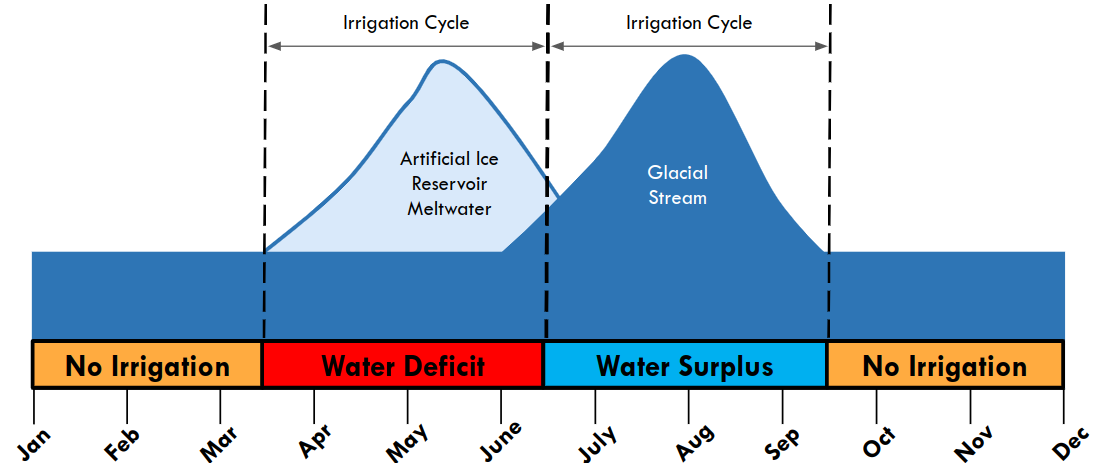
\includegraphics[width=12cm]{Figures/irrigation_cycles.png}

\caption{Seasonal variation in the availability of irrigation water. The graph highlights the crucial role of
AIRs in bridging the critical gap in water availability. Adapted from: \cite{nusserLocalKnowledgeGlobal2016}}

\label{fig:irrigation_cycles}
\end{figure}

Cryosphere-fed irrigation networks in arid mountain regions are completely dependent on timely availability of
meltwater from glaciers, snow and permafrost \citep{immerzeelImportanceVulnerabilityWorld2020,
farhanHydrologicalRegimesConjunction2015, tveitenGlacierGrowingLocal2007}. With the accelerated decline of
glaciers due to climate change \citep{nusserLocalKnowledgeGlobal2016}, these regions are experiencing water
scarcity particularly during the spring season \citep{norphelSnowWaterHarvesting2015,
mukhopadhyayReevaluationSnowmeltGlacial2015} (see Fig. \ref{fig:irrigation_cycles}). This seasonal water
scarcity makes it essential to provide supplementary irrigation in order to sustain agricultural output and take
advantage of the complete growing season \citep{nusserLocalKnowledgeGlobal2016, vincentEnergyClimateChange2009}.

To cope with this recurrent water scarcity, villagers in the region of Ladakh have developed two types of
artificial ice reservoirs (AIRs): ice stupas and ice terraces.  All these types of ice reservoirs capture water
in the autumn and winter, allowing it to freeze, and hold it until spring, when it melts and flows down to
fields \citep{ipccChapterHighMountain2019, vinceGlacierMan2009, clouseLadakhArtificialGlaciers2017,
nusserSociohydrologyArtificialGlaciers2019}. In this way, they retain a previously unused portion of the annual
flow and facilitate its use to supplement the decreased flow in the following spring (see Fig.
\ref{fig:irrigation_cycles}). This study focuses on the form of AIRs locally called as ice stupas.

Over the past decade, several ice stupas have been built to supplement irrigation water supply of mountain
villages in India \citep{wangchukIceStupaCompetition2020, palmerStoringFrozenWater2022,
aggarwalAdaptationClimateChange2021}, Kyrgyzstan \citep{bbcnewsBrightArtificialGlacier2020} and Chile
\citep{reutersConservationistsChileAim2021}. Despite this widespread adoption, only a few publications examine
the role of AIRs in the water resource management of these regions. None of these publications study AIRs
outside Ladakh. Moreover, the published quantifications of the water storage capacity of AIRs just in Ladakh
also vary widely between these studies \citep{norphelSnowWaterHarvesting2015, baglaArtificialGlaciersHelp1998}.

Quantifying the water storage capacity of AIRs is not straightforward since the formative processes of AIRs are
complex. These processes are controlled by local topography, meteorology and construction strategies used. Since
AIRs are ice structures with similar surface processes like glaciers, glacier models could be used to quantify
meteorological influences. However, due to their limited size, and comparatively more variable surface area,
this assessment requires a modelling approach which is optimally constrained with comprehensive data from
in-situ field measurements. Moreover, a spirit of improvisation guides the design and construction of AIRs
making it difficult to make quantitative comparison from site to site.  

This thesis fulfills these requirements as it provides a new set of AIR-specific volume and area measurements
from drone flights along with meteorological data during the construction period. All these datasets were
produced through construction strategies using fountain systems that are quantified via in-situ observations of
the fountain characteristics and discharge rate measurements. This thesis also provides a one-dimensional AIR
model which is calibrated and validated with several AIR datasets from locations with different meteorological
conditions and different fountain systems. While this thesis reviews published AIR research and presents a
comprehensive quantitative study of their water storage potential, we acknowledge that substantial additional
knowledge is held by farming communities building these structures since mid-1800s.

\begin{figure}[t]
\centering
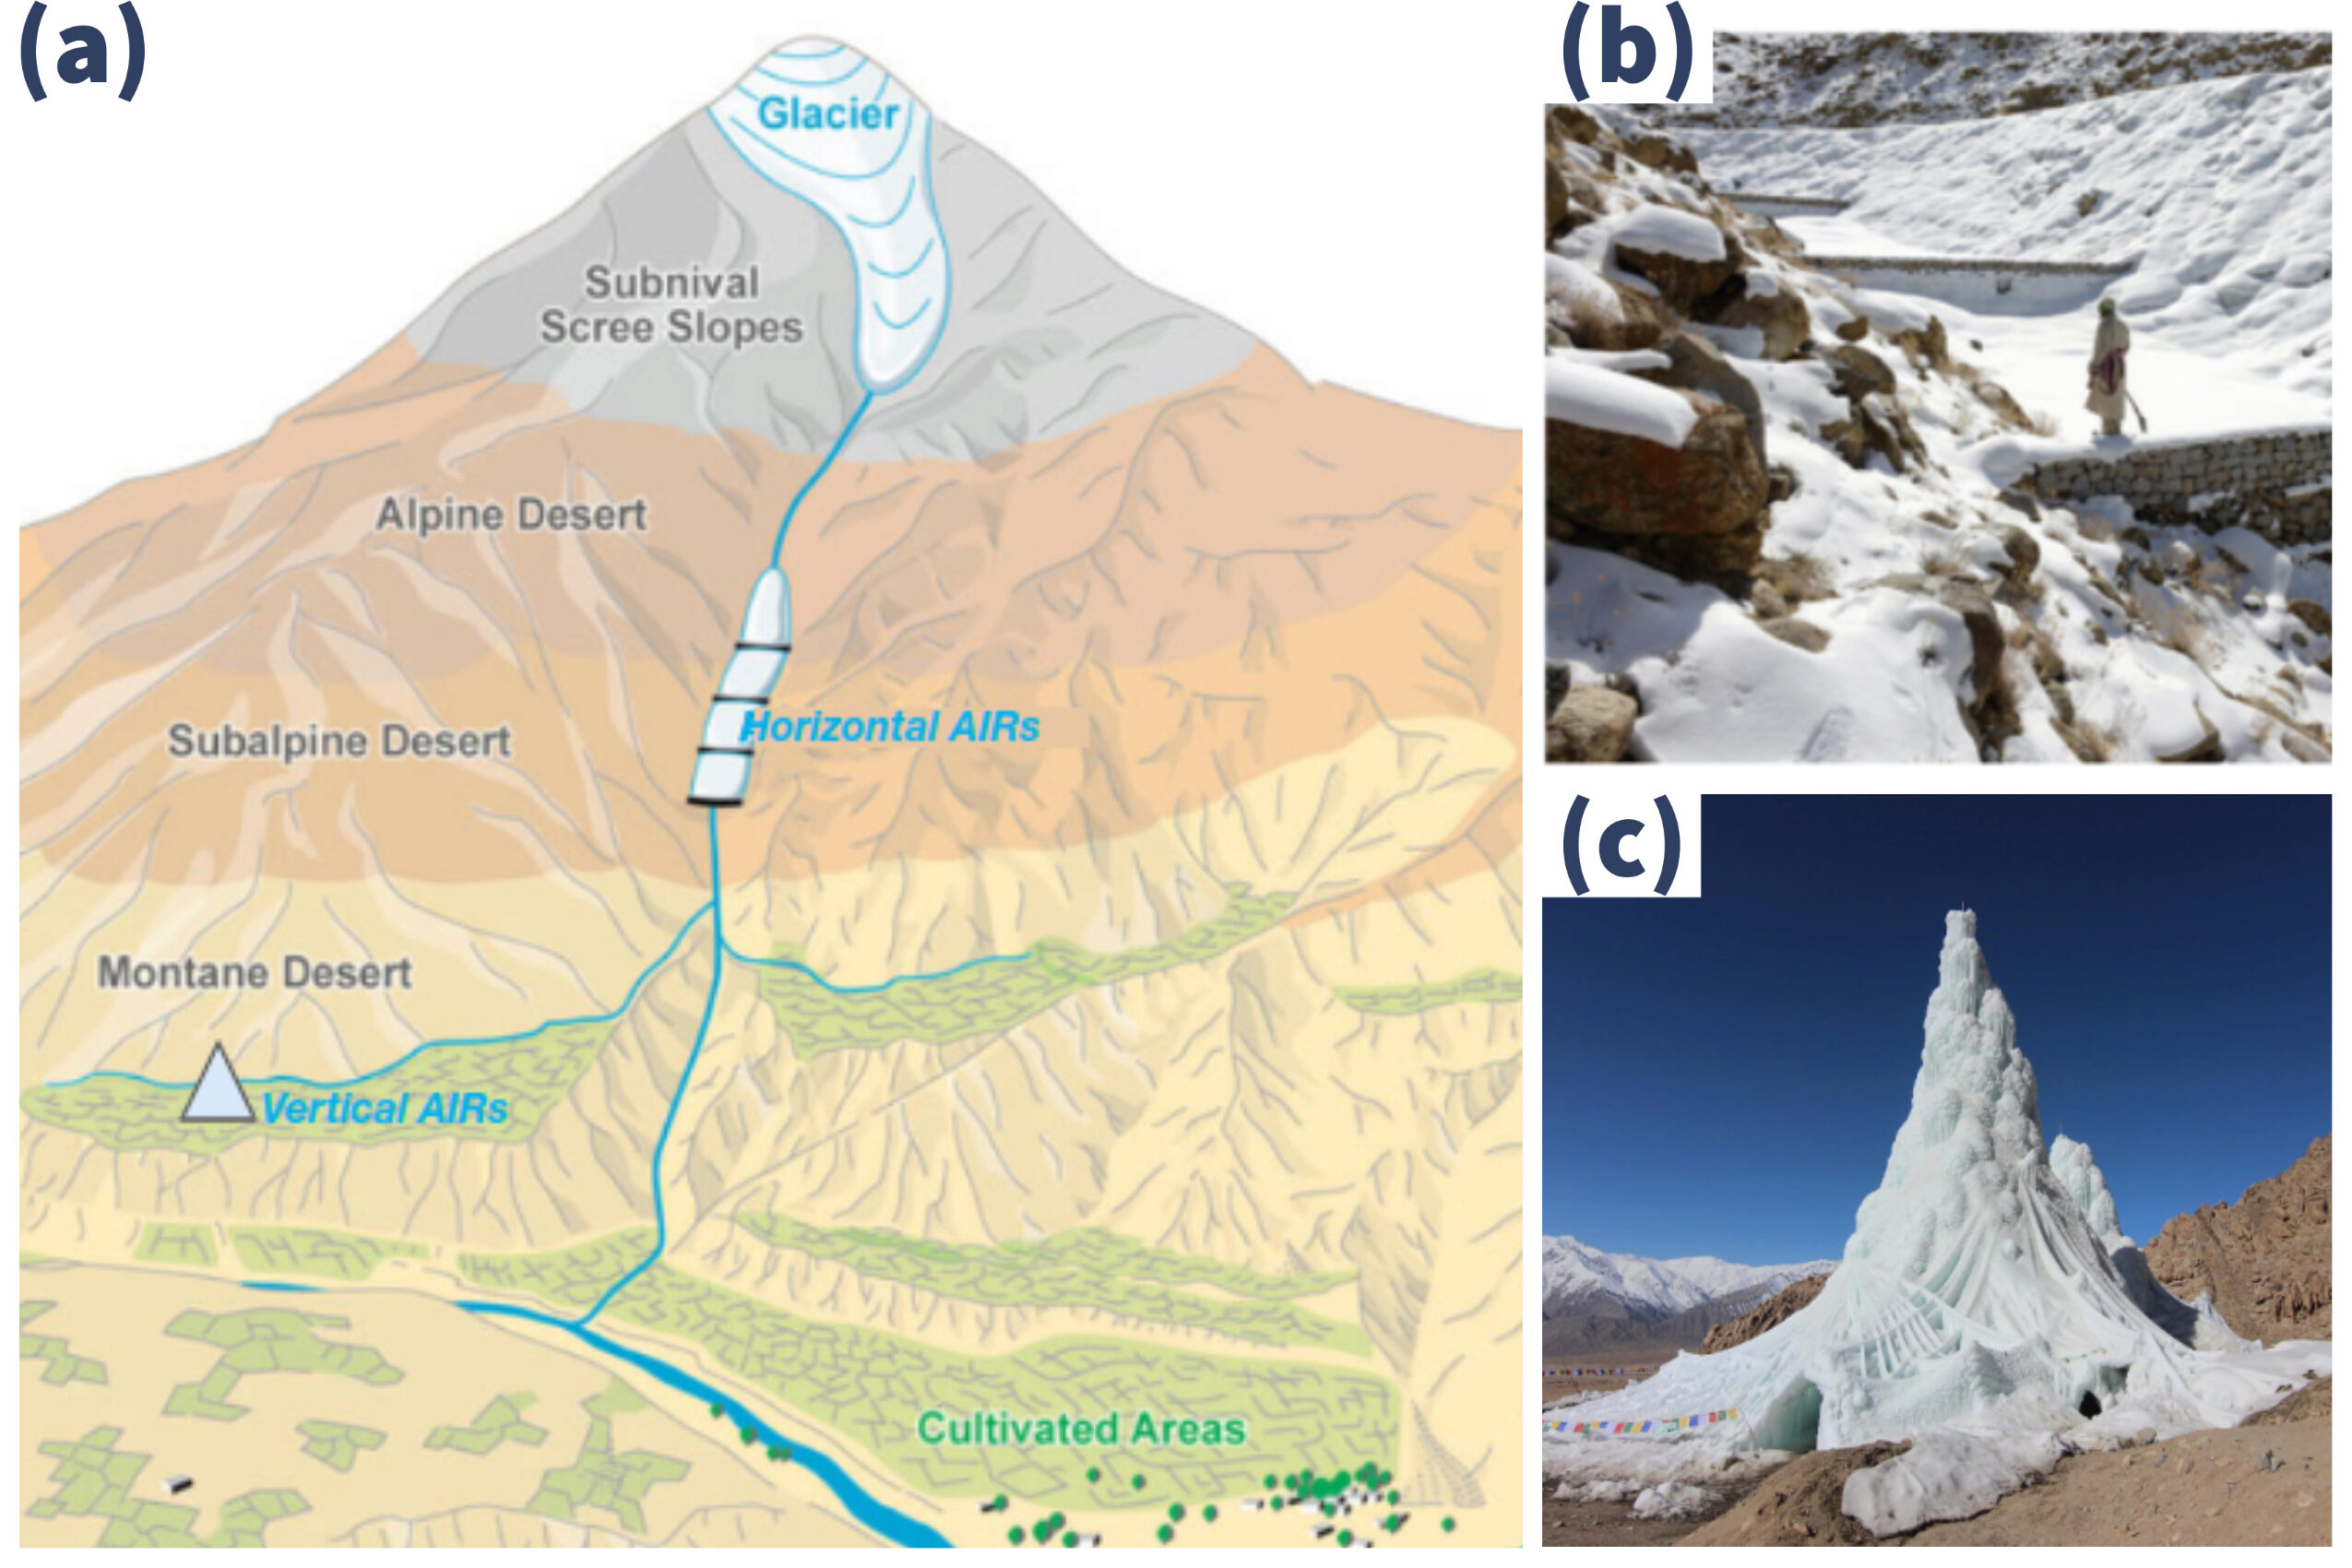
\includegraphics[width=12cm]{Figures/AIR_forms.jpg}

\caption{(a) Schematic overview of the position of artificial ice reservoirs. These constructions are located at
  altitudes between the glaciers and the irrigation networks in the cultivated areas. (b) Ice terraces at 3900
  m, located above the village of Nang, Ladakh. The cascade is composed of a series of loose masonry walls
  ranging in height from 2 to 3 $m$, which help freeze water for storage. (c) Ice stupas at 3600 m, located
above the village of Phyang, Ladakh. They are made using fountain systems. Adapted from:
\cite{nusserLocalKnowledgeGlobal2016}}

\label{fig:AIRforms}
\end{figure}

\section{Nomenclature and Classification}

In spite of the popularity of the term "artificial glacier", we deliberately use the term "ice reservoir" since
it conveys character and function of these structures more accurately
\citep{nusserSociohydrologyArtificialGlaciers2019}. Man-made ice structures typically have a lifetime in the
order of months and a size million times smaller than typical glaciers. Therefore, any comparison between these
ice structures can be misleading. Since glaciers are considered as natural ice reservoirs, we use the
terminology artificial ice reservoirs (AIRs) to distinguish man-made ice structures described in this thesis. 

A spirit of improvisation guides the construction strategy of AIRs making it difficult to classify them.
However, it has been found that construction strategies using fountain systems form AIRs which tend towards a
conical shape and those without form flat sheets of ice. Therefore, this thesis classifies all the AIRs produced
based on whether or not they use fountain systems. AIRs using fountain systems are called "ice stupas" and those
without are called "ice terraces" since this terminology denotes the resulting shape of the respective AIRs
appropriately.

\section{Objectives}

The main objective of this thesis is to quantify the water storage potential of AIRs based on the construction
site and fountain chosen. 

An integrated study approach including field measurements and modelling is applied to answer the following
research questions: 

\begin{enumerate}

\item What is the influence of construction location and fountain characteristics on AIR volume evolution? 

\item How can ice stupa fountain systems be engineered to reduce water loss and maintenance of AIRs?

\end{enumerate}

An energy and mass balance model for artificial ice reservoirs was set up to answer the first research question
(paper I and II). Since in-situ measurements were required to run this model, a measurement campaign was
executed in Switzerland and India during the past 4 winters. These datasets provided the necessary input,
calibration and validation data to model the evolution of AIRs and study their sensitivity to meteorological
conditions and fountain characterestics (paper II). 

Two weather-sensitive construction strategies were developed to answer the second research question. These
construction strategies employed fountains whose discharge rate was regulated by automation system using the AIR
model developed before. Their advantages and disadvantages over traditional construction strategy are quantified
in paper III.

\section{Structure}

Chapter 1 introduces the motivation of this work and provides a summary of the state of knowledge about AIRs
prior to this thesis. Chapter 2 describes the origins of this technology as a religious practice. Chapter 3
gives an overview about the study sites and introduces the different field techniques applied. The influence of
the construction location through its meteorological and topographical conditions are presented in Chapter 4.
The engineering design of AIR technologies are showcased in Chapter 5 along with suggestions for their
improvement. Chapter 6 concludes the thesis with a synthesis and future outlook. Papers I, II and III are
included in the Appendix.


 % Introduction

% \input{Chapters/Literature} % Background Theory

\chapter{Methods}


\section{Data Collection}

We chose two villages in the Swiss Alps and the Indian Himalayas called Guttannen and Gangles to collect the
required datasets described above. These two locations exhibit drastically different weather patterns (see
Table) owing to their latitude, longitude and altitude differences. This enabled us to highlight the
meteorological influences on ice volume evolution (RQ 1).

The Guttannen site (46.66 $\degree$N, 8.29 $\degree$E) is situated in the Berne region, Switzerland and has an
altitude of 1047 $m$ a.s.l. In the winter (Oct-Apr), mean daily minimum and maximum air temperatures vary
between -13 and 15 $\degree C$. Clear skies are rare, averaging around 7 days during winter. Daily winter
precipitation can sometimes be as high as 100 $mm$. These values are based on 30 years of hourly historical
weather data measurements \citep{meteoblueClimateGuttannen2021}. Several AIRs were constructed by the Guttannen
Bewegt Association, the University of Fribourg and the Lucerne University of Applied Sciences and Arts during
the winters of 2020-22.

The Gangles site (34.22 $\degree$N, 77.61 $\degree$E) is located around 20 km north of Leh city in the Ladakh
region, lying at 4025 $m$ a.s.l.. The mean annual temperature is $5.6 \, \degree C$, and the thermal range is
characterized by high seasonal variation. During January, the coldest month, the mean temperature drops to $-7.2
\, \degree C$. During August, the warmest month, the mean temperature rises to $17.5 \, \degree C$
\citep{Nusser_2012}. Because of the rain shadow effect of the Himalayan Range, the mean annual precipitation in
Leh totals less than 100 $mm$, and there is high interannual variability. Whereas the average summer rainfall
between July and September reaches 37.5 $mm$, the average winter precipitation between January and March amounts
to 27.3 $ mm$ and falls almost entirely as snow. AIRs were constructed here as part of the Ice Stupa Competition
by the Himalayan Institute of Alternatives, Ladakh (HIAL). 


 % Experimental Setup

%\input{Chapters/Chapter4} % Experiment 1

%\chapter{Conclusions}

Chapter 5 provides conclusions based on research findings from data collected on AIRs in Switzerland and India,
as well as discussion and recommendations for future research. This Chapter will review the purpose of the
study, research questions, literature review, and findings of the study. It will then present conclusions,
discussion of the conclusions, and recommendations for practice and for further research.

\section{Summary}

Cryosphere fed irrigation networks are completely dependant on the timely availability of meltwater from
glaciers, snow and permafrost. With the accelerated decline of glaciers, these irrigation networks have failed
to deliver adequate water to sustain agricultural output and take advantage of the complete growing season. As a
consequence, many mountain villages have either been abandoned or lie on the brink of desertification.

In the past few decades, artificial ice reservoir (AIR) technologies have provided much needed relief to these
water-stressed communities. These strategies revolve around augmenting their glacial ice reservoirs with
man-made ones that provide supplementary irrigation during the spring. From folklore to science, from art to
technology, these practices of reclaiming glacial water have come a long way. 

Empirical data and studies focussing on AIRs are sparse. Depending on the relative influence of weather
conditions and fountain characteristics, AIRs typically show high variability in their ice volume dynamics.
Because small-scale processes, complex feedbacks and non-linearities govern their evolution, accessing the
response of AIRs to the location and fountain chosen is challenging and only feasible if backed up with
comprehensive field data. In the context of the observed present and predicted global glacier shrinkage, the
development of such water storage technologies is crucial to ensure continued survival of mountain communities.

\section{Conclusions}

The main objective of this thesis was thus to improve our understanding about the response of AIRs to changes in
their construction location and fountain characteristics. With a special focus on icestupas, here defined as
vertical AIRs, volume changes were investigated in detail based on the comparison of weather patterns, fountain
characteristics and volume observations between several AIRs. A mass and energy model was created which allowed
ice volume estimation of icestupas. AIR radius, area and volume were recorded using DEMs produced from drone
flights. The fountain characteristics were calibrated from the observed radius and discharge rates. The model
parameters were calibrated from some volume observations. The rest of this DEM dataset were used to validate the
modelled volume evolution. The ice volume dynamics due to the difference in weather patterns of the Swiss
location and Indian location can be summarised as follows: 

% \begin{itemize} 

% \item[\tiny{$\blacksquare$}] Colder temperatures and lower humidity led to higher sublimation and lower
%   conduction.
%  
% \item[\tiny{$\blacksquare$}] Cloudy days increase shortwave radiation impact.
%  
% \end{itemize}

\begin{itemize} 

\item[\tiny{$\blacksquare$}] Icestupa's volume evolution depends on meteorological conditions and fountain
  characteristics.

\item[\tiny{$\blacksquare$}] Icestupas gain volume due to higher vapour losses and not inspite of it. 

\item[\tiny{$\blacksquare$}] Icestupa's shape decreases direct shortwave radiation impact.

\item[\tiny{$\blacksquare$}] Icestupas gain volume due to higher vapour losses and not inspite of it. 

\item[\tiny{$\blacksquare$}] Icestupas suffer high water losses.
 
\end{itemize}

\begin{itemize} 

\item[\tiny{$\blacksquare$}] Colder, drier and less cloudy construction locations form long-lasting AIRs with
  higher maximum ice volumes. 

\item[\tiny{$\blacksquare$}] Fountains that produce smaller droplets form larger AIRs with higher slope. 

\end{itemize}


\section{Discussion}

\section{Recommendations}

\section{Suggestions for future research}

\section{Final thoughts}
 % Experiment 2

%\input{Chapters/Chapter6} % Results and Discussion

\chapter{Conclusions}

Chapter 5 provides conclusions based on research findings from data collected on AIRs in Switzerland and India,
as well as discussion and recommendations for future research. This Chapter will review the purpose of the
study, research questions, literature review, and findings of the study. It will then present conclusions,
discussion of the conclusions, and recommendations for practice and for further research.

\section{Summary}

Cryosphere fed irrigation networks are completely dependant on the timely availability of meltwater from
glaciers, snow and permafrost. With the accelerated decline of glaciers, these irrigation networks have failed
to deliver adequate water to sustain agricultural output and take advantage of the complete growing season. As a
consequence, many mountain villages have either been abandoned or lie on the brink of desertification.

In the past few decades, artificial ice reservoir (AIR) technologies have provided much needed relief to these
water-stressed communities. These strategies revolve around augmenting their glacial ice reservoirs with
man-made ones that provide supplementary irrigation during the spring. 

Summary of the literature review

From folklore to science, from art to technology, these practices of reclaiming glacial water have come a long
way. 

Empirical data and studies focussing on AIRs are sparse. Depending on the relative influence of weather
conditions and fountain characteristics, AIRs typically show high variability in their ice volume dynamics.
Because small-scale processes, complex feedbacks and non-linearities govern their evolution, accessing the
response of AIRs to the location and fountain chosen is challenging and only feasible if backed up with
comprehensive field data. 

Summary of the methodology

In the context of the observed present and predicted global glacier shrinkage, the development of such water
storage technologies is crucial to ensure continued survival of mountain communities.

Summary of the findings

\section{Conclusions}

The main objective of this thesis was thus to improve our understanding about the response of AIRs to changes in
their construction location and fountain characteristics. With a special focus on icestupas, here defined as
vertical AIRs, volume changes were investigated in detail based on the comparison of weather patterns, fountain
characteristics and volume observations between several AIRs. A mass and energy model was created which allowed
ice volume estimation of icestupas. AIR radius, area and volume were recorded using DEMs produced from drone
flights. The fountain characteristics were calibrated from the observed radius and discharge rates. The model
parameters were calibrated from some volume observations. The rest of this DEM dataset were used to validate the
modelled volume evolution. The ice volume dynamics due to the difference in weather patterns of the Swiss
location and Indian location can be summarised as follows: 

% \begin{itemize} 

% \item[\tiny{$\blacksquare$}] Colder temperatures and lower humidity led to higher sublimation and lower
%   conduction.
%  
% \item[\tiny{$\blacksquare$}] Cloudy days increase shortwave radiation impact.
%  
% \end{itemize}

\begin{itemize} 

\item[\tiny{$\blacksquare$}] Icestupa's volume evolution depends on meteorological conditions and fountain
  characteristics.

\item[\tiny{$\blacksquare$}] Icestupas gain volume due to higher vapour losses and not inspite of it. 

\item[\tiny{$\blacksquare$}] Icestupa's shape decreases direct shortwave radiation impact.

\item[\tiny{$\blacksquare$}] Icestupas gain volume due to higher vapour losses and not inspite of it. 

\item[\tiny{$\blacksquare$}] Icestupas suffer high water losses.
 
\end{itemize}

\begin{itemize} 

\item[\tiny{$\blacksquare$}] Colder, drier and less cloudy construction locations form long-lasting AIRs with
  higher maximum ice volumes. 

\item[\tiny{$\blacksquare$}] Fountains that produce smaller droplets form larger AIRs with higher slope. 

\end{itemize}


\section{Discussion}

\section{Recommendations}

\section{Suggestions for future research}

\section{Final thoughts}
 % Conclusion

%% ----------------------------------------------------------------
% Now begin the Appendices, including them as separate files

\addtocontents{toc}{\vspace{2em}} % Add a gap in the Contents, for aesthetics

\appendix % Cue to tell LaTeX that the following 'chapters' are Appendices

% \chapter{An Appendix}

Lorem ipsum dolor sit amet, consectetur adipiscing elit. Vivamus at pulvinar nisi. Phasellus hendrerit, diam placerat interdum iaculis, mauris justo cursus risus, in viverra purus eros at ligula. Ut metus justo, consequat a tristique posuere, laoreet nec nibh. Etiam et scelerisque mauris. Phasellus vel massa magna. Ut non neque id tortor pharetra bibendum vitae sit amet nisi. Duis nec quam quam, sed euismod justo. Pellentesque eu tellus vitae ante tempus malesuada. Nunc accumsan, quam in congue consequat, lectus lectus dapibus erat, id aliquet urna neque at massa. Nulla facilisi. Morbi ullamcorper eleifend posuere. Donec libero leo, faucibus nec bibendum at, mattis et urna. Proin consectetur, nunc ut imperdiet lobortis, magna neque tincidunt lectus, id iaculis nisi justo id nibh. Pellentesque vel sem in erat vulputate faucibus molestie ut lorem.

Quisque tristique urna in lorem laoreet at laoreet quam congue. Donec dolor turpis, blandit non imperdiet aliquet, blandit et felis. In lorem nisi, pretium sit amet vestibulum sed, tempus et sem. Proin non ante turpis. Nulla imperdiet fringilla convallis. Vivamus vel bibendum nisl. Pellentesque justo lectus, molestie vel luctus sed, lobortis in libero. Nulla facilisi. Aliquam erat volutpat. Suspendisse vitae nunc nunc. Sed aliquet est suscipit sapien rhoncus non adipiscing nibh consequat. Aliquam metus urna, faucibus eu vulputate non, luctus eu justo.

Donec urna leo, vulputate vitae porta eu, vehicula blandit libero. Phasellus eget massa et leo condimentum mollis. Nullam molestie, justo at pellentesque vulputate, sapien velit ornare diam, nec gravida lacus augue non diam. Integer mattis lacus id libero ultrices sit amet mollis neque molestie. Integer ut leo eget mi volutpat congue. Vivamus sodales, turpis id venenatis placerat, tellus purus adipiscing magna, eu aliquam nibh dolor id nibh. Pellentesque habitant morbi tristique senectus et netus et malesuada fames ac turpis egestas. Sed cursus convallis quam nec vehicula. Sed vulputate neque eget odio fringilla ac sodales urna feugiat.

Phasellus nisi quam, volutpat non ullamcorper eget, congue fringilla leo. Cras et erat et nibh placerat commodo id ornare est. Nulla facilisi. Aenean pulvinar scelerisque eros eget interdum. Nunc pulvinar magna ut felis varius in hendrerit dolor accumsan. Nunc pellentesque magna quis magna bibendum non laoreet erat tincidunt. Nulla facilisi.

Duis eget massa sem, gravida interdum ipsum. Nulla nunc nisl, hendrerit sit amet commodo vel, varius id tellus. Lorem ipsum dolor sit amet, consectetur adipiscing elit. Nunc ac dolor est. Suspendisse ultrices tincidunt metus eget accumsan. Nullam facilisis, justo vitae convallis sollicitudin, eros augue malesuada metus, nec sagittis diam nibh ut sapien. Duis blandit lectus vitae lorem aliquam nec euismod nisi volutpat. Vestibulum ornare dictum tortor, at faucibus justo tempor non. Nulla facilisi. Cras non massa nunc, eget euismod purus. Nunc metus ipsum, euismod a consectetur vel, hendrerit nec nunc.	% Appendix Title

%\input{Appendices/AppendixB} % Appendix Title

%\input{Appendices/AppendixC} % Appendix Title

\addtocontents{toc}{\vspace{2em}}  % Add a gap in the Contents, for aesthetics
\backmatter

%% ----------------------------------------------------------------
\label{Bibliography}
\lhead{\emph{Bibliography}}  % Change the left side page header to "Bibliography"
\bibliographystyle{unsrtnat}  % Use the "unsrtnat" BibTeX style for formatting the Bibliography
\bibliography{zot_refs}  % The references (bibliography) information are stored in the file named "Bibliography.bib"

\end{document}  % The End
%% ----------------------------------------------------------------
